\documentclass[11pt,a4paper]{article}

\usepackage[margin=2.5cm, headheight=15pt]{geometry}
\usepackage{graphicx}
\usepackage{caption}
\usepackage{subcaption}
\usepackage{booktabs}
\usepackage{xcolor}
\usepackage{enumitem}
\usepackage{titlesec}
\usepackage{hyperref}
\usepackage{fancyhdr}
\usepackage{tabularx}
\usepackage{array}
\usepackage{float}
\usepackage{multicol}
\usepackage{tcolorbox}
\tcbuselibrary{skins}

\setlength{\parskip}{6pt}
\setlength{\parindent}{0pt}

\definecolor{deadred}{HTML}{C0392B}
\definecolor{deadgold}{HTML}{D4AC0D}
\definecolor{deadgray}{HTML}{2C3E50}
\definecolor{deaddark}{HTML}{1A1A2E}
\definecolor{lightgray}{HTML}{F0F0F0}

\titleformat{\section}{\large\bfseries\color{deadred}}{}{0em}{}[\color{deadgray}\titlerule]
\titleformat{\subsection}{\normalsize\bfseries\color{deadgray}}{}{0em}{}
\titlespacing{\section}{0pt}{14pt}{6pt}
\titlespacing{\subsection}{0pt}{10pt}{4pt}

\pagestyle{fancy}
\fancyhf{}
\lhead{\textcolor{deadgray}{\small\textit{Deadlight: Survival After Dark}}}
\rhead{\textcolor{deadgray}{\small\textit{Deliverable 3 -- Final Report}}}
\cfoot{\textcolor{deadgray}{\small\thepage}}
\renewcommand{\headrulewidth}{0.4pt}

\hypersetup{colorlinks=true, linkcolor=deadred, urlcolor=deadred}
\captionsetup{font=small, labelfont={bf,color=deadgray}, textfont=it}

\tcbset{
  tableframe/.style={
    colback=lightgray,
    colframe=deadgray,
    boxrule=0.5pt,
    arc=2pt,
    left=8pt, right=8pt, top=6pt, bottom=6pt
  }
}

% ===================================================================
\begin{document}

% ===================================================================
%  TITLE PAGE
% ===================================================================
\begin{titlepage}
  \pagecolor{deaddark}
  \color{white}
  \vspace*{3cm}
  \begin{center}
    {\fontsize{38}{46}\selectfont\bfseries\textcolor{deadred}{DEADLIGHT}}\\[0.3cm]
    {\Large\textcolor{deadgold}{Survival After Dark}}\\[1.2cm]
    \textcolor{deadgray}{\rule{0.6\textwidth}{0.6pt}}\\[0.8cm]
    {\large\bfseries Deliverable 3: Final Game Prototype}\\[0.2cm]
    {\large\bfseries and Showcase Presentation}\\[0.6cm]
    \textcolor{deadgray}{\rule{0.6\textwidth}{0.6pt}}\\[1.2cm]
    {\normalsize
      \textbf{Course:} CS4483B / 9541 Game Design\\[0.3cm]
      \textbf{Group:} 16\\[0.3cm]
      \textbf{Members:}\\[0.2cm]
      Simranjeet Singh \quad Abdelrahman El Banna\\
      Koroush Emari \quad Ashraf Esam Mahdi\\[0.6cm]
      \textbf{Date:} April 2026
    }
  \end{center}
  \vfill
  \begin{center}
    \textcolor{deadgold}{\small\textit{``The evacuation failed. You didn't.''}}
  \end{center}
\end{titlepage}
\nopagecolor

% ===================================================================
%  TABLE OF CONTENTS
% ===================================================================
\tableofcontents
\newpage

% ===================================================================
%  1. PROJECT OVERVIEW
% ===================================================================
\section{Project Overview}

\textit{Deadlight: Survival After Dark} is a top-down 2D zombie survival game built in Unity. The player controls a lone survivor moving through four environments (Town Center, Suburban, Industrial, and Research Facility), each containing three campaign nights, for a total of twelve nights across four levels.

Each session cycles through three phases. The \textbf{Day Phase} involves exploration, story objectives, and supply collection. The \textbf{Night Phase} involves defending against escalating enemy waves and responding to optional helicopter drops. The \textbf{Dawn Phase} is a shop screen where the player spends earned points on weapons, armour, and upgrades before the next night. A narrative arc involving Project Lazarus, EVAC Command, and a mutant subject called Subject~23 is delivered through radio messages, lore collectibles, and scripted story beats across all four levels.

\textbf{Deliverable 3 scope.} Deliverable 2 covered Levels 1 and 2. For Deliverable 3, the team completed Levels 3 and 4 with new maps and story content, added a three-phase boss fight against Subject~23, introduced a run modifier system for replay variation, implemented dynamic audio mixing, added a run-grading and leaderboard system, and performed a full playtesting and balance pass across all twelve nights.

\begin{figure}[H]
  \centering
  \begin{subfigure}[t]{0.48\textwidth}
    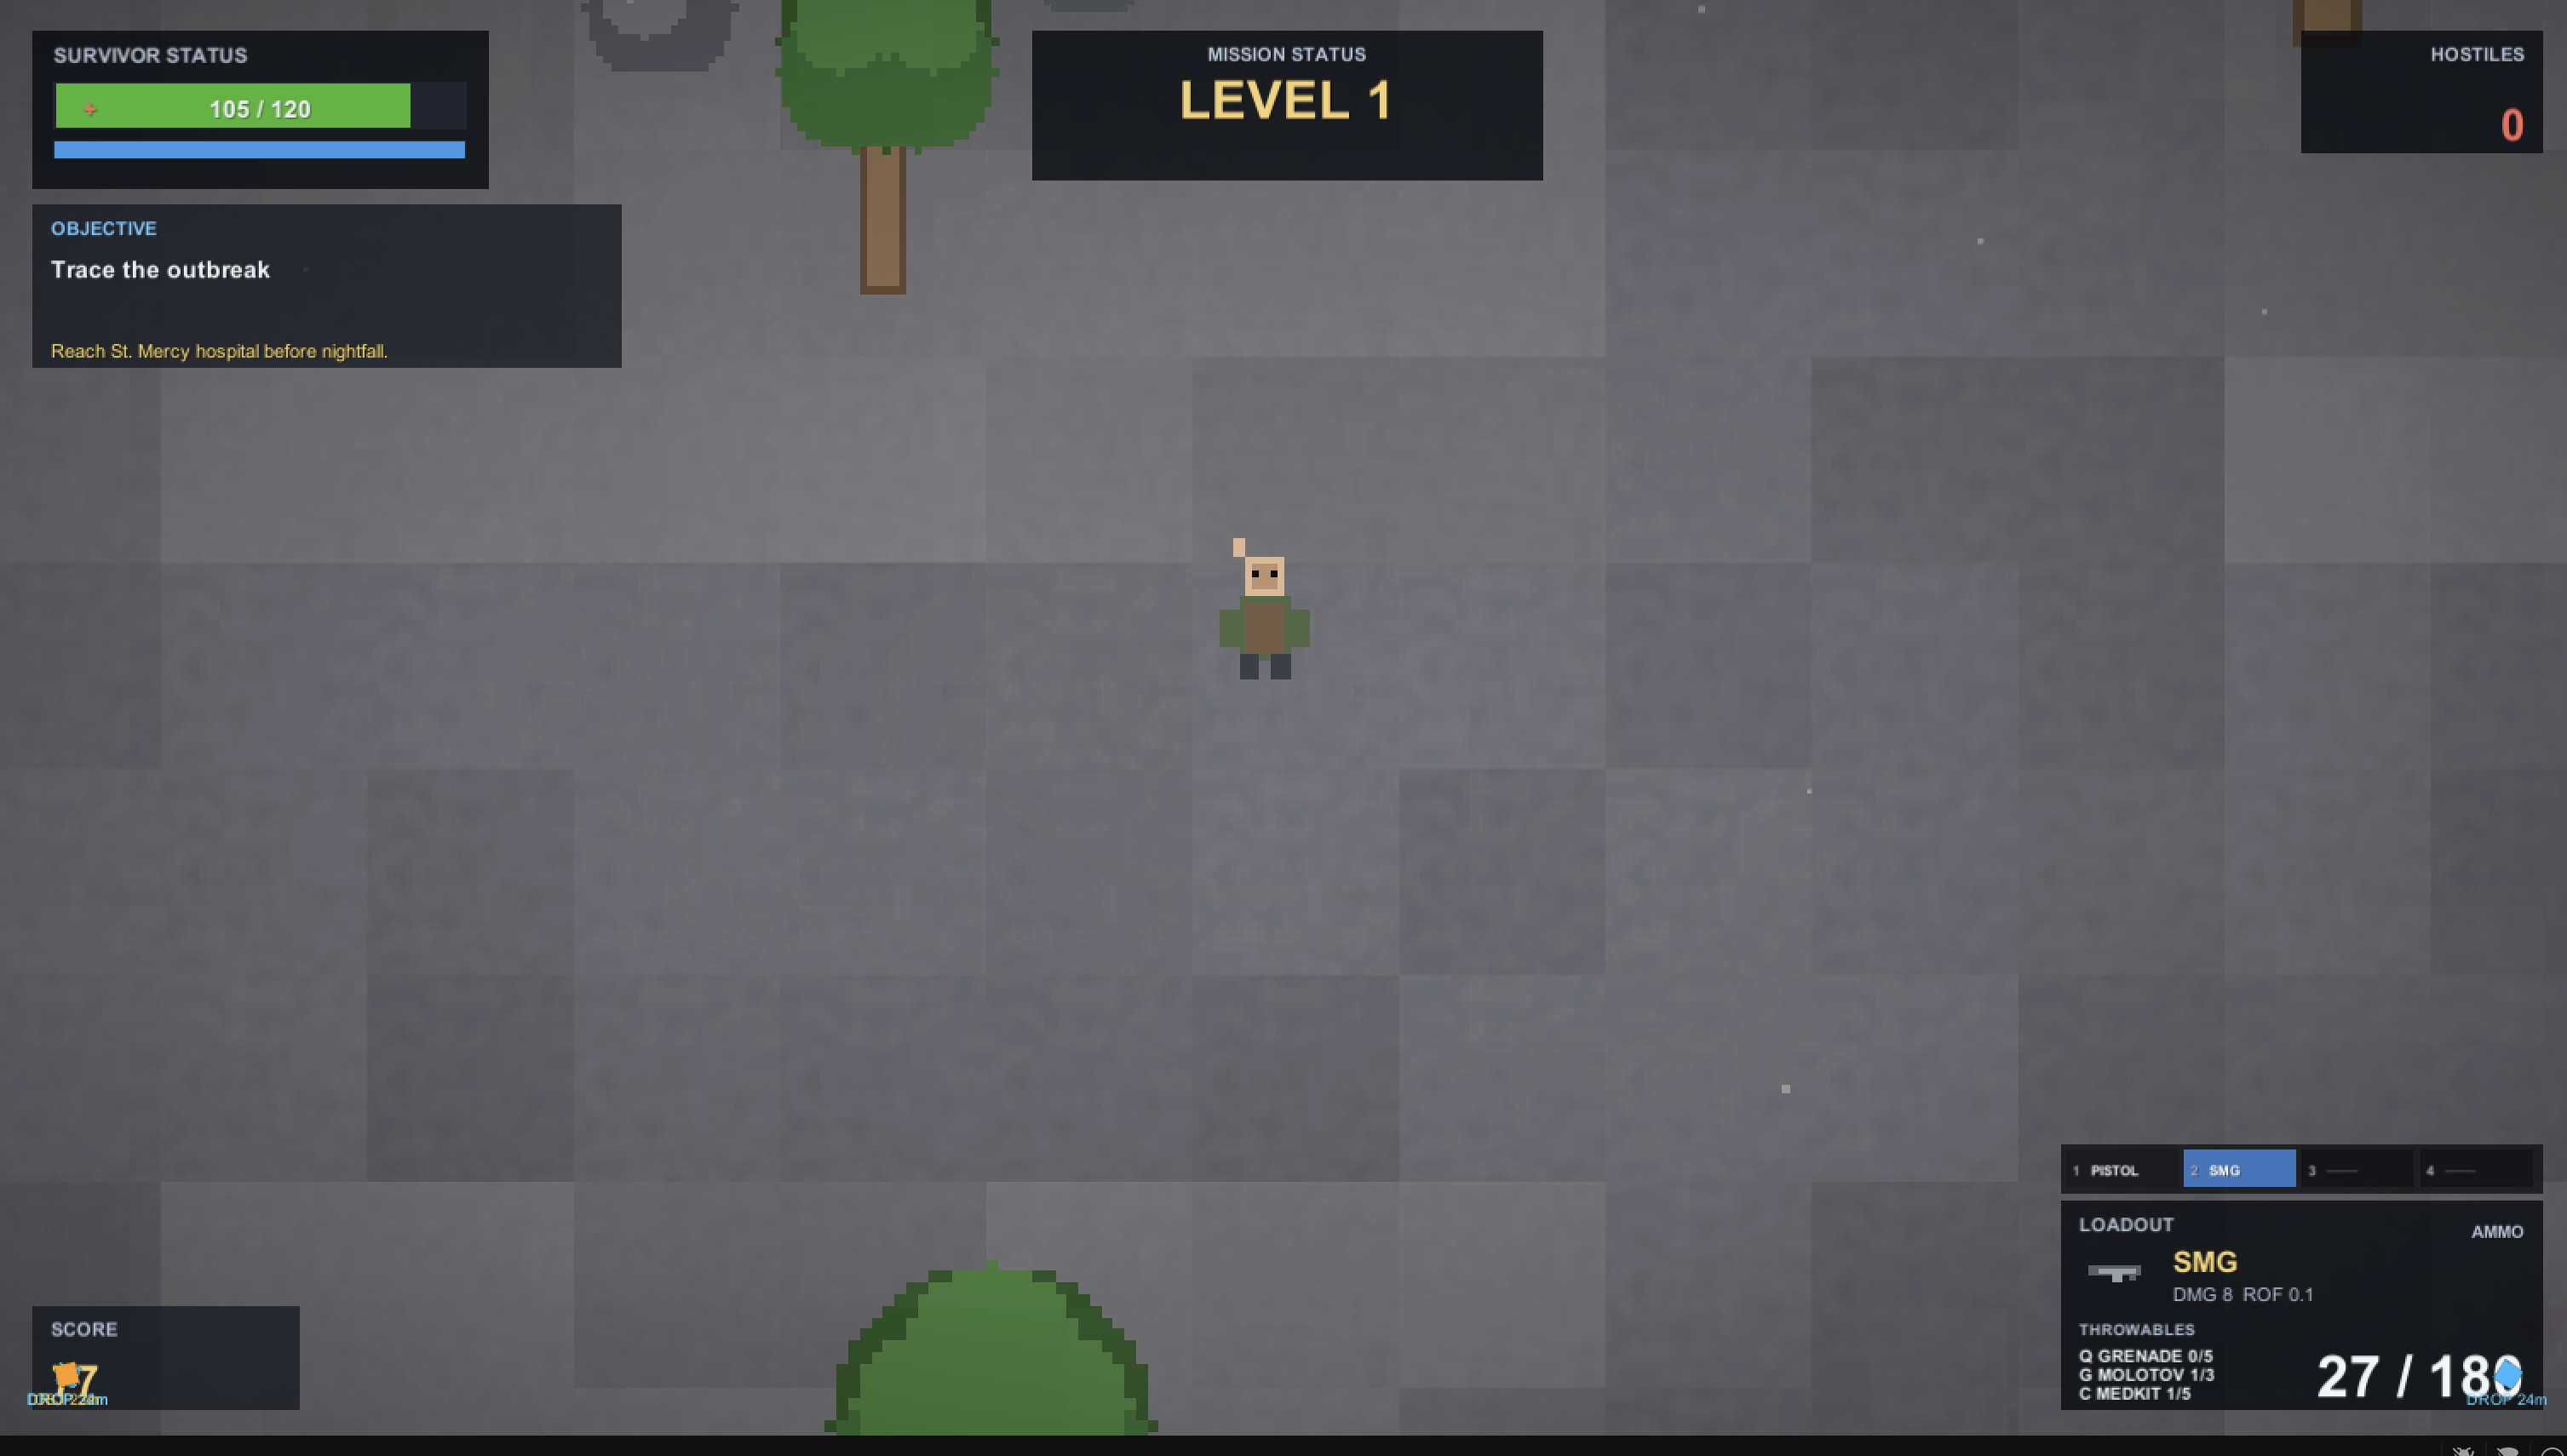
\includegraphics[width=\textwidth]{d2_fig_hud.png}
    \caption{Daytime exploration in Level 1 (Town Center). The HUD shows health, armour, active objective, loadout, ammo, and score.}
  \end{subfigure}
  \hfill
  \begin{subfigure}[t]{0.48\textwidth}
    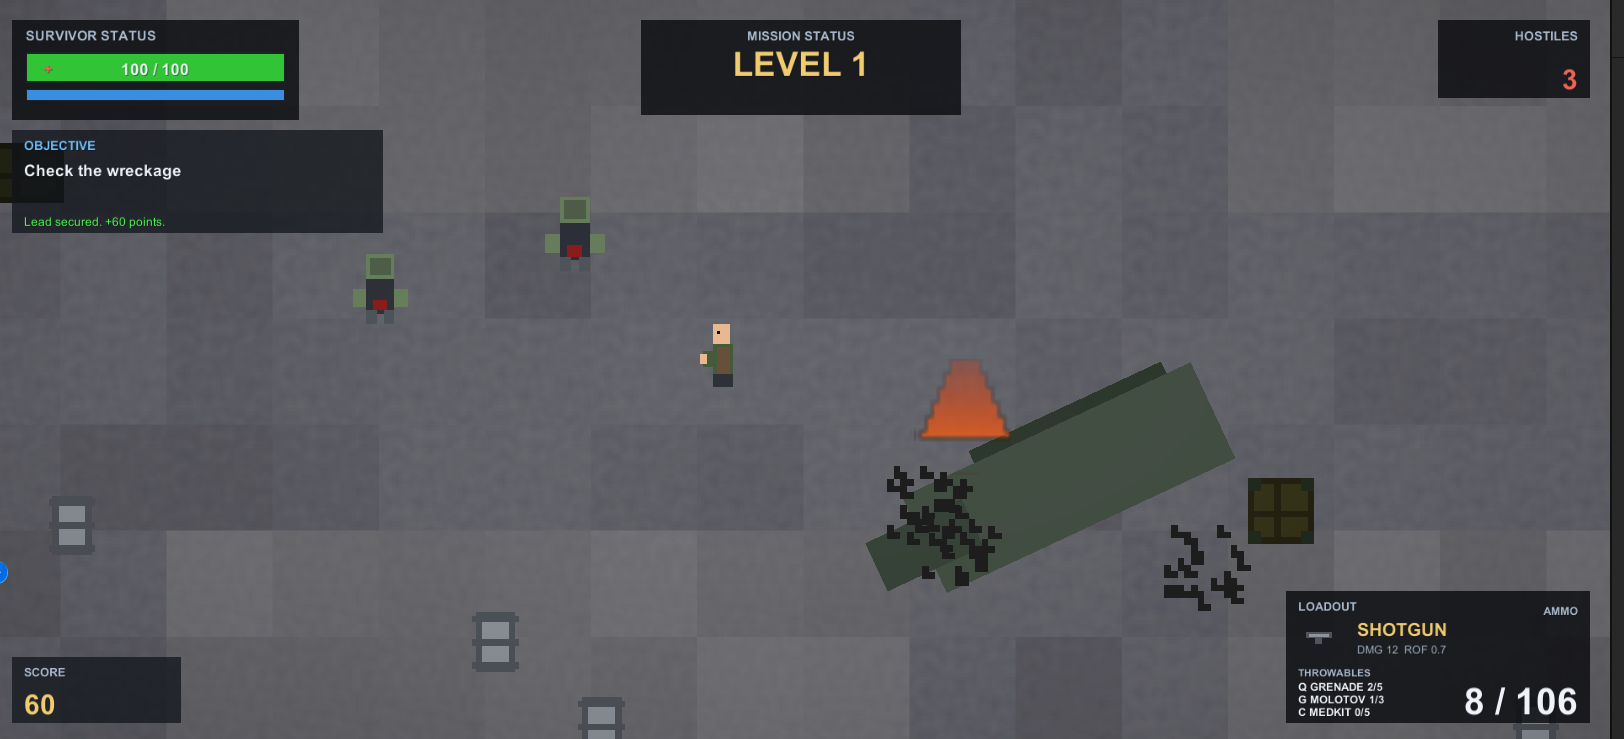
\includegraphics[width=\textwidth]{d2_fig_combat.png}
    \caption{Night Phase combat in Level 1, Wave 2. Blood decals, wave counter, and hostile tracker are visible.}
  \end{subfigure}
\end{figure}

% ===================================================================
%  2. ART, AESTHETICS & SOUND DESIGN
% ===================================================================
\section{Art, Aesthetics \& Sound Design}

\subsection{Visual Direction}

The game uses a muted top-down pixel art style. Building tiles and road surfaces use a desaturated grey-green base. Accent colours are used only where they carry meaning: gold for objectives and supply drops, red for danger, and blue for interactive objects. This keeps the environment easy to read during combat.

\textbf{Procedural sprites.} All character and prop sprites are generated at runtime by \texttt{ProceduralSpriteGenerator}. The player sprite includes armour overlays that change colour based on the equipped vest tier. Enemy sprites share a base zombie shape with per-type colour tints and size variations. The boss spawns at twice the standard enemy scale. Supply crates use three colour codes: \textbf{Common} (brown), \textbf{Rare} (blue), and \textbf{Legendary} (gold), allowing the player to identify crate quality from a distance.

\textbf{Bullet trail.} Each bullet uses an 8-pixel sprite with a bright centre fading to orange at the edge, combined with a \texttt{TrailRenderer} set to fade over 55~ms. This makes projectile direction and speed readable without dedicated art assets.

\textbf{Atmosphere.} \texttt{AtmosphereController} applies a colour tint over the scene that shifts between a warm tone during the day and a dark blue during the night, in sync with the day-night timer. \texttt{VFXManager} handles screen shake and muzzle flash effects. \texttt{DecalManager} places blood marks on the ground when enemies are killed. These marks remain visible for the rest of the night, giving areas where combat occurred a distinct appearance.

\begin{figure}[H]
  \centering
  \begin{subfigure}[t]{0.48\textwidth}
    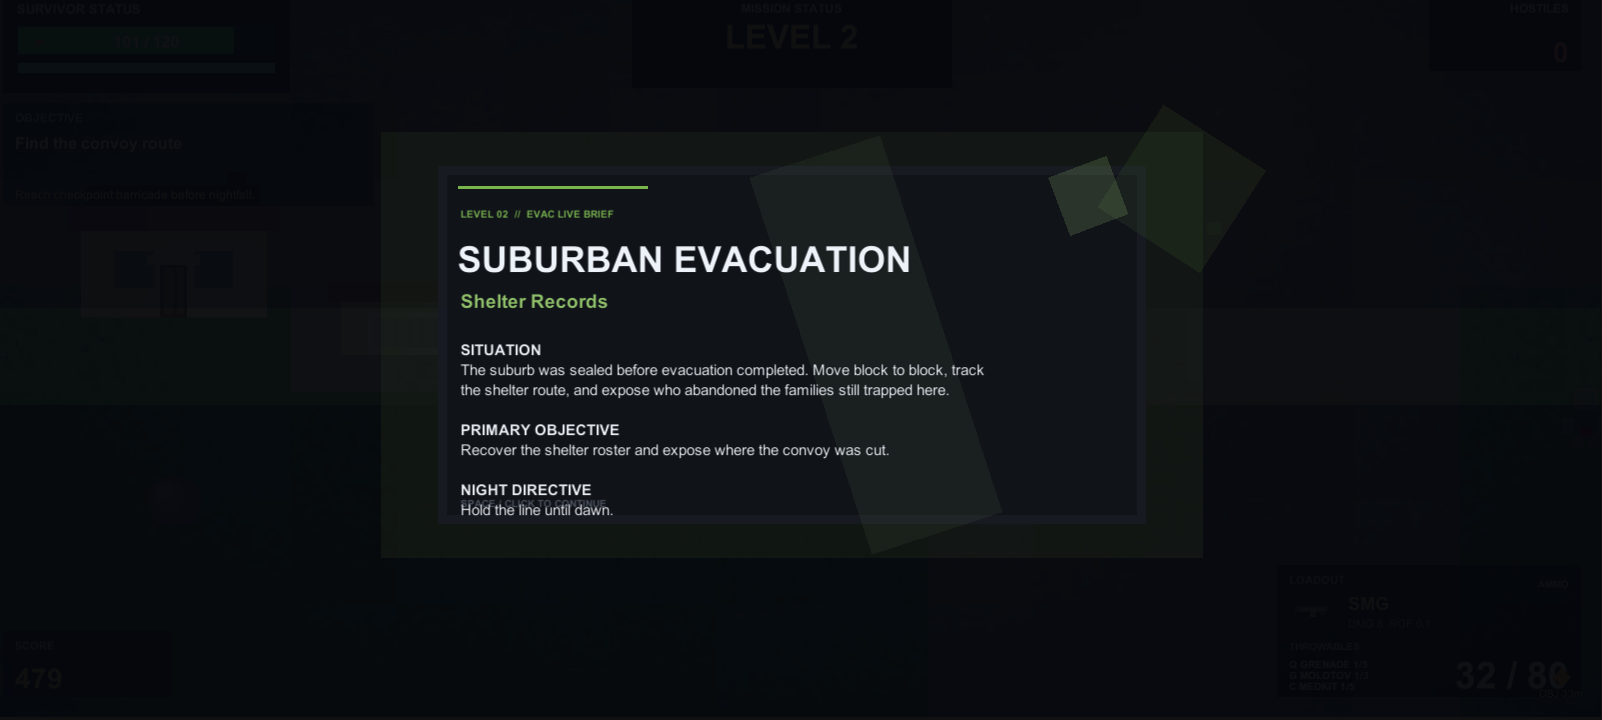
\includegraphics[width=\textwidth]{d2_fig_level2_briefing.png}
    \caption{Contested day drop in Level 2. The objective ring, COMMS message, and supply crate are all visible at the same time.}
  \end{subfigure}
  \hfill
  \begin{subfigure}[t]{0.48\textwidth}
    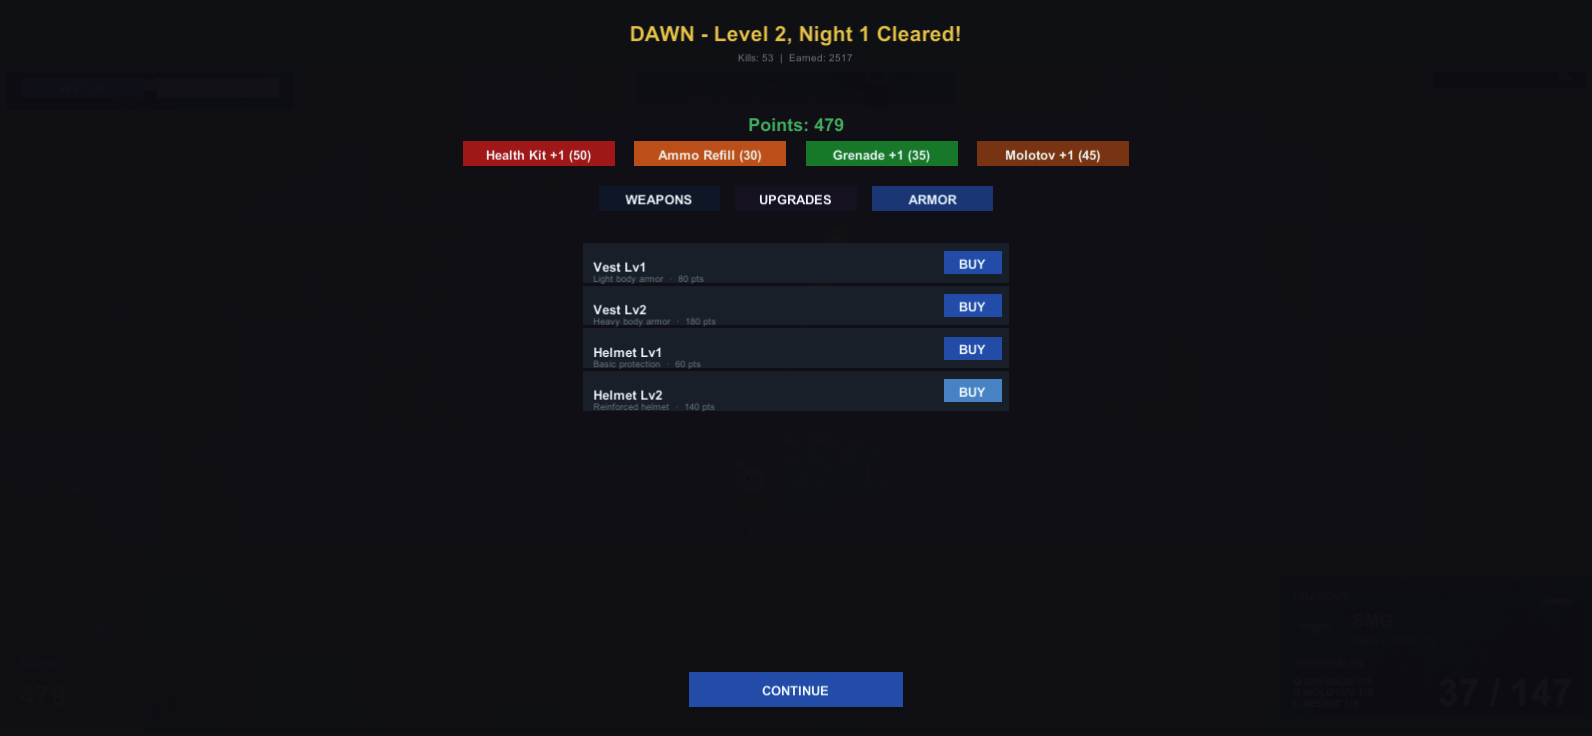
\includegraphics[width=\textwidth]{d2_fig_dawn_shop_v2.png}
    \caption{Dawn Shop after Level 2, Night 1. Points total, consumable row, and tabbed shop panels (Weapons / Upgrades / Armour) are shown.}
  \end{subfigure}
\end{figure}

\begin{figure}[H]
  \centering
  \begin{subfigure}[t]{0.48\textwidth}
    \includegraphics[width=\textwidth]{d3_fig_industrial_overview.png}
    \caption{Level 3 (Industrial) overview capture generated from the runtime map builder. Wide lanes and dense cover pockets support higher-pressure mid-campaign nights.}
  \end{subfigure}
  \hfill
  \begin{subfigure}[t]{0.48\textwidth}
    \includegraphics[width=\textwidth]{d3_fig_research_overview.png}
    \caption{Level 4 (Research) overview capture. The layout tightens into corridors and chokepoints around the final objective sector.}
  \end{subfigure}
\end{figure}

\subsection{User Interface}

The HUD is divided into five fixed areas on screen:

\begin{itemize}[noitemsep]
  \item \textbf{Top-left:} Health bar, armour bar, active objective, and COMMS feed.
  \item \textbf{Top-centre:} Level name and wave number during the night, or phase label during the day.
  \item \textbf{Top-right:} Enemy count and, when a helicopter drop is scheduled, a countdown timer.
  \item \textbf{Bottom-right:} Weapon slots, active weapon stats, throwable counts, and current ammo.
  \item \textbf{Bottom-left:} Score.
\end{itemize}

\texttt{UITheme} stores shared fonts, colours, and panel sizes so that all runtime-created panels use the same style. The Dawn shop uses three tabs (Weapons, Upgrades, Armour) with a row of consumable buttons above them.

\subsection{Sound Design}

\texttt{AudioManager} handles five music tracks (menu, day, night, boss, dawn) and crossfades between them over 3.2 seconds when the game state changes. A tension value is updated at runtime based on the current phase (\texttt{dayBaseTension = 0.05}, \texttt{nightBaseTension = 0.28}, \texttt{bossBaseTension = 0.80}). This value is used to adjust music volume, pitch, and ambient level so that the audio mix becomes more intense as waves progress.

A pool of ten \texttt{AudioSource} components handles spatial sound effects such as gunfire, enemy sounds, and explosions, with a range of 20 metres. \texttt{ProceduralAudioGenerator} produces pickup and interaction sounds at runtime. When radio dialogue or COMMS messages play, the background music volume is reduced by 24\% so the speech remains audible.

% ===================================================================
%  3. NARRATIVE & SYSTEMS INTEGRATION
% ===================================================================
\section{Narrative \& Systems Integration}

\subsection{Story Arc}

The campaign follows a containment story across four levels. Each level takes place in a different environment and advances a distinct part of the narrative.

\begin{tcolorbox}[tableframe]
\small
\begin{tabularx}{\textwidth}{@{} l l X @{}}
\toprule
\textbf{Level} & \textbf{Map} & \textbf{Story content} \\
\midrule
1 & Town Center & The evacuation has failed. The player makes first contact with EVAC Command and finds early signs of Project Lazarus at a crash site, checkpoint, and clinic. \\
2 & Suburban & Quarantine records are discovered. Lore drops reveal details of the Lazarus research programme. \\
3 & Industrial & A Lazarus laboratory is confirmed. Intercepted communications from Dr.\ Chen document the collapse of the supply chain. \\
4 & Research Facility & The player fights to contain Subject~23 in a three-phase boss encounter. EVAC extraction is triggered if Subject~23 is defeated. \\
\bottomrule
\end{tabularx}
\end{tcolorbox}

\begin{figure}[H]
  \centering
  \begin{subfigure}[t]{0.48\textwidth}
    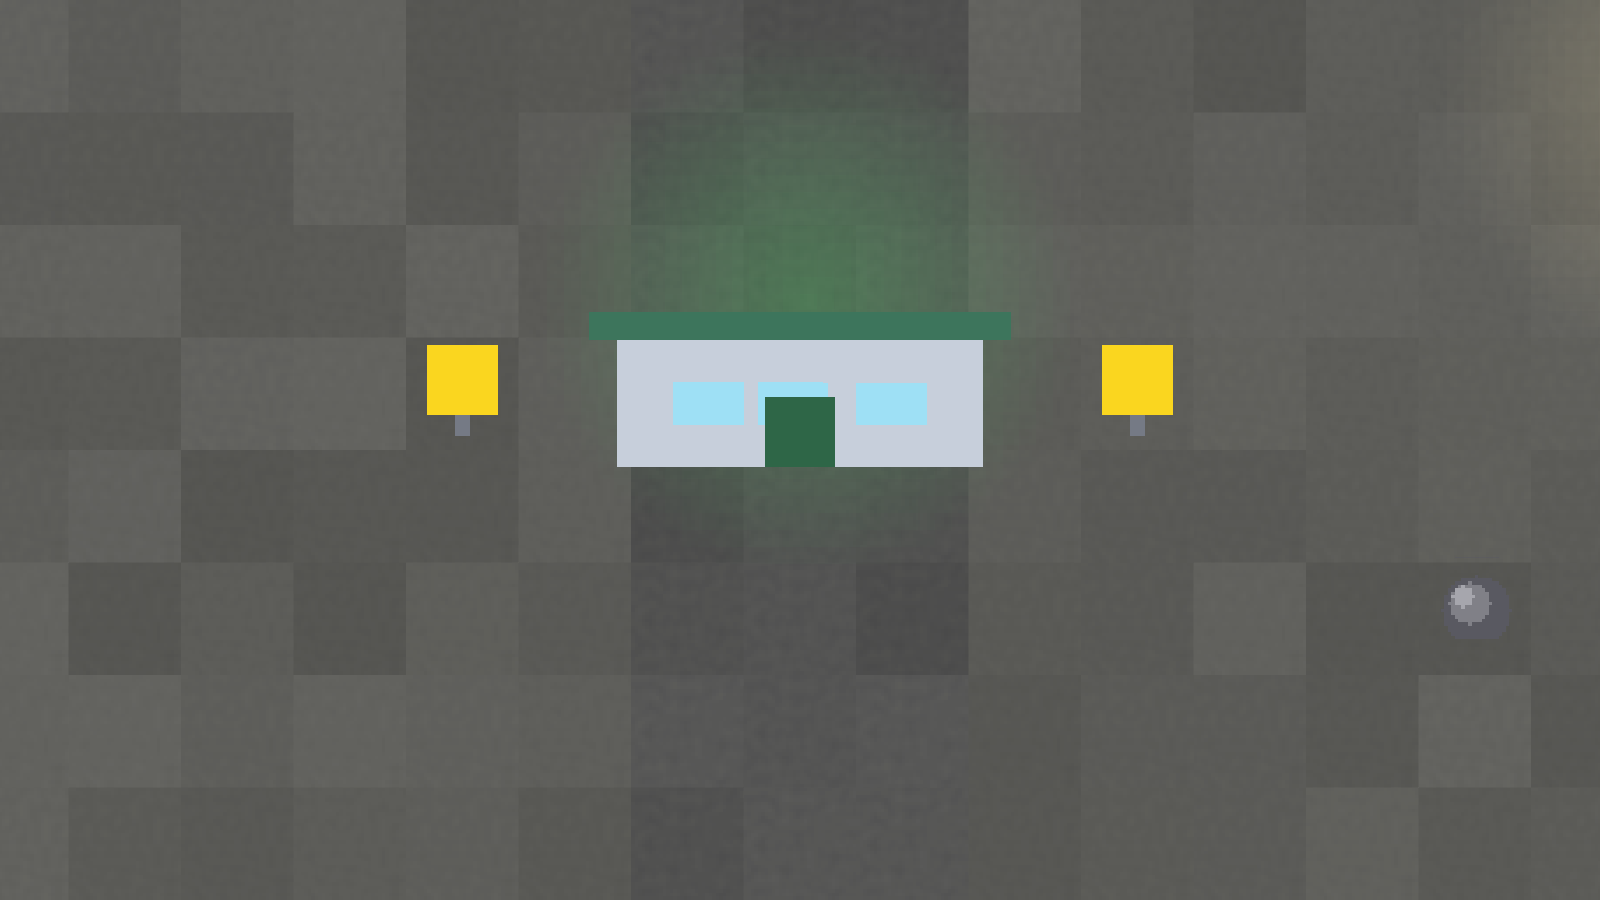
\includegraphics[width=\textwidth]{d3_fig_industrial_lab.png}
    \caption{Industrial laboratory zone used in Level 3 objective beats and lore discovery paths.}
  \end{subfigure}
  \hfill
  \begin{subfigure}[t]{0.48\textwidth}
    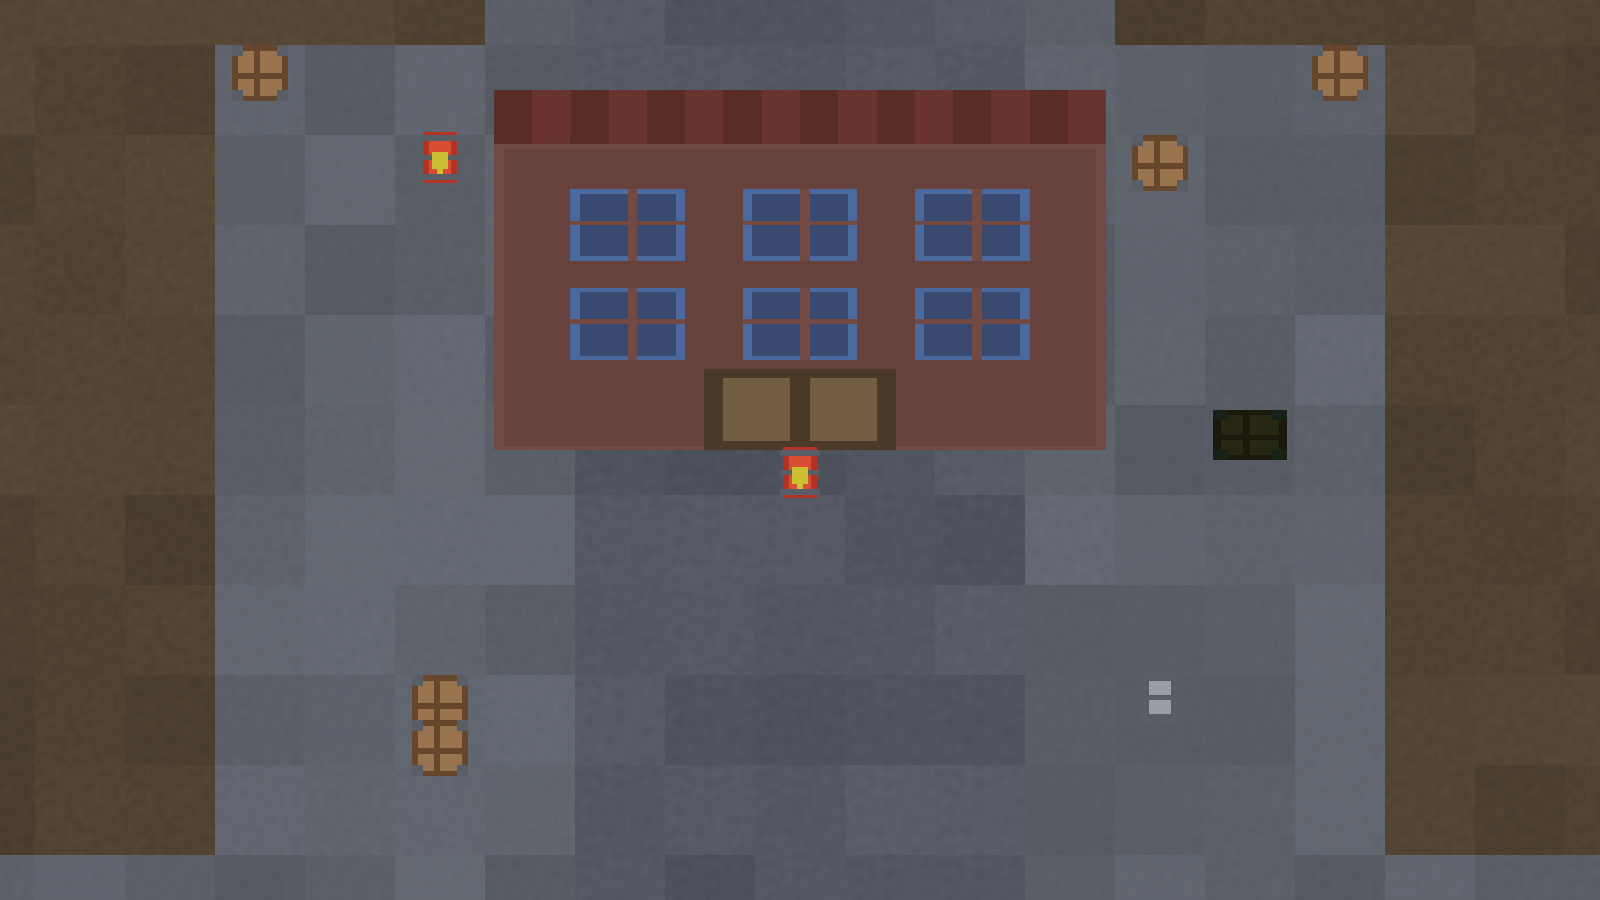
\includegraphics[width=\textwidth]{d3_fig_research_reactor_yard.png}
    \caption{Research reactor yard pathing in Level 4, used to pressure player movement during late-night encounters.}
  \end{subfigure}
\end{figure}

\subsection{Narrative Delivery}

The player can complete every night without engaging with the story. All narrative content is optional or ambient, delivered through the following systems.

\textbf{Radio / COMMS.} \texttt{RadioTransmissions} queues messages from EVAC Command, Dr.~Chen, and survivor voices. A 1.2-second protection window prevents a new message from interrupting one that is already playing. The message appears in a panel above the objective display with a channel label.

\textbf{Story Objectives.} \texttt{StoryObjective} assigns a title, description, and two-phase structure (Day Investigation, then Night Survival) to each of the twelve campaign nights. Completed entries are stored in a list and displayed in \texttt{NarrativeJournalUI}, which the player can open at any time.

\textbf{Environmental lore.} \texttt{EnvironmentalLore} and \texttt{LorePickup} place optional items such as graffiti, lab notes, and survivor logs across each map. These do not affect progression. The Level Complete screen reports a lore count (for example, ``Lore Found: 0/25'') as a secondary metric.

\textbf{Player voice.} \texttt{PlayerVoice} triggers short audio reactions tied to gameplay events such as low health, a first kill, or seeing the boss. The clips are generated procedurally.

\subsection{Narrative Consequences in Gameplay}

Failing a story objective has mechanical effects. A missed \texttt{StoryObjective} adds a \textbf{1.2x enemy strength multiplier} to the following night and reduces the point carryover into the next level by a \textbf{0.75x penalty}. Both effects are announced through COMMS messages that distinguish between a retry and a forced advance. Contested day drops follow the same pattern: EVAC Command announces the drop by radio, an objective marker shows the location, and the outcome (secured or lost) is reported back through COMMS.

\begin{figure}[H]
  \centering
  \begin{subfigure}[t]{0.48\textwidth}
    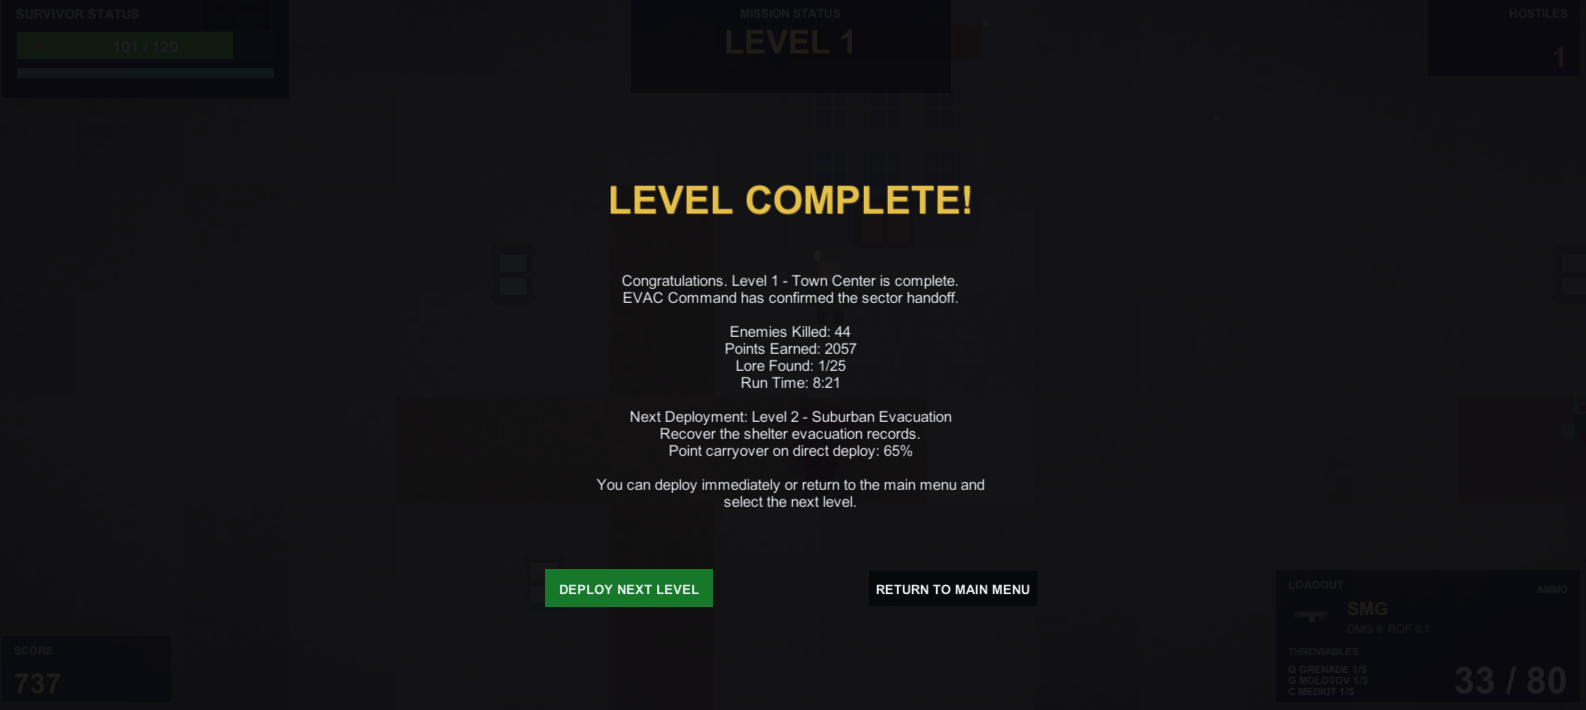
\includegraphics[width=\textwidth]{d2_fig_level1_complete.png}
    \caption{Level Complete panel after Level 1. The next deployment is identified by name, and lore count is shown as a secondary completion metric.}
    \label{fig:levelcomplete}
  \end{subfigure}
  \hfill
  \begin{subfigure}[t]{0.48\textwidth}
    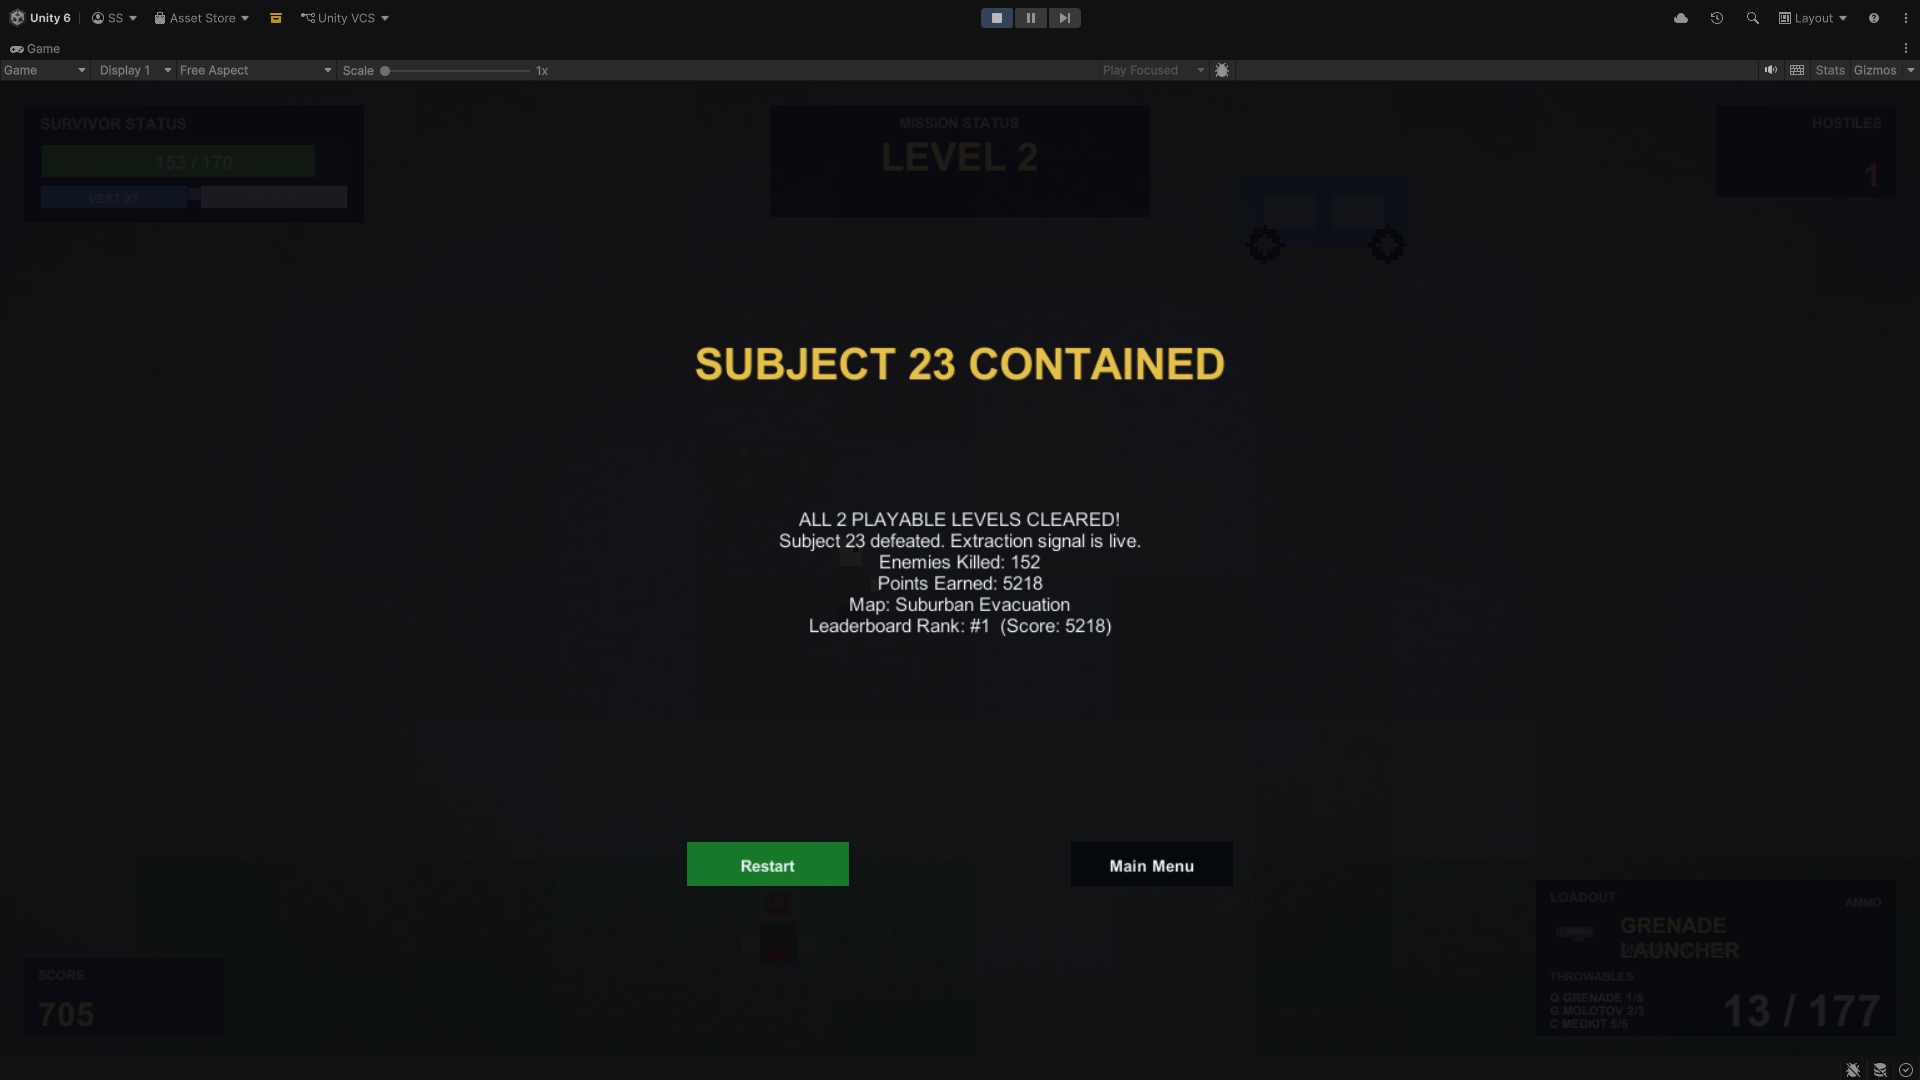
\includegraphics[width=\textwidth]{d2_fig_victory.png}
    \caption{Victory screen after defeating Subject 23. Kill count, points, map name, and leaderboard rank are displayed.}
  \end{subfigure}
\end{figure}

% ===================================================================
%  4. PROGRESSION & BALANCE
% ===================================================================
\section{Progression \& Balance}

\subsection{Campaign Structure}

The campaign is structured as four levels, each containing three nights. Level access is tracked in \texttt{PlayerPrefs} using two keys (\texttt{Deadlight\_UnlockedLevel} and \texttt{Deadlight\_HighestCompletedLevel}). A player can return to any previously completed level but cannot skip ahead. \texttt{GameManager.IsLevelUnlocked()} enforces this by comparing the requested level against the highest completed level plus one.

Each level starts with a full reset of points, inventory, weapon loadout (pistol only), armour, throwables, and medkits. Within a level, the player builds up resources across three nights and spends them at the Dawn shop between nights.

\subsection{Night Pacing}

Day and night durations are set individually for each of the twelve nights.

\begin{center}
\small
\begin{tabular}{@{} l c c @{}}
\toprule
\textbf{Level (nights)} & \textbf{Day duration (s)} & \textbf{Night duration (s)} \\
\midrule
Level 1 (N1--3) & 90, 80, 70 & 55, 65, 80 \\
Level 2 (N4--6) & 85, 75, 65 & 55, 70, 85 \\
Level 3 (N7--9) & 80, 70, 60 & 65, 80, 100 \\
Level 4 (N10--12) & 75, 65, 55 & 80, 100, 140 \\
\bottomrule
\end{tabular}
\end{center}

Day phases become shorter in later levels, reducing preparation time. Night phases become longer, increasing the time the player must hold out against enemies. Enemy statistics are not changed between levels; pacing is handled through duration alone.

\subsection{Adaptive Resource Scaling}

The number of health and ammo pickups spawned each day decreases slightly across levels. Ammo pickup counts are also adjusted at runtime based on the player's current reserve ammo.

\begin{tcolorbox}[tableframe]
\small
\begin{tabular}{@{} l c c c c @{}}
\toprule
\textbf{Resource} & \textbf{Level 1} & \textbf{Level 2} & \textbf{Level 3} & \textbf{Level 4} \\
\midrule
Health pickups & 4 & 4 & 3 & 3 \\
Ammo pickups (base) & 5 & 5 & 4 & 4 \\
\bottomrule
\end{tabular}

\vspace{6pt}
\textbf{Ammo pickup count adjustment by reserve ammo:} \\
Reserve $\geq 320$: no pickups spawned. \quad Reserve $\geq 240$: 25\% of base count. \\
Reserve $\geq 160$: 50\% of base count. \quad Below 160: full count spawns.
\end{tcolorbox}

Pickups are placed using a 100-attempt scatter algorithm. It biases positions toward the outer 40\% of the map, enforces a minimum 6-unit gap between pickups, rejects positions within 10 units of the player spawn point, and checks all obstacle colliders to avoid placing pickups inside buildings.

\subsection{Supply Crate Tiers and Helicopter Drops}

Crates come in three tiers. The probability of higher tiers increases with the campaign night number.

\[
P(\mathrm{Legendary}) = \min(0.12,\ 0.01 + 0.01 \times \mathrm{night}), \quad
P(\mathrm{Rare}) = \min(0.35,\ 0.08 + 0.02 \times \mathrm{night})
\]

Night helicopter drops have a 65\% base spawn chance, reduced if the player's ammo reserve is already high. The drop is scheduled after a 55-second delay with up to 8 seconds of randomisation. Contested day drops trigger at 68\% through the day phase, with a 60\% base chance that is reduced at high ammo reserves.

\subsection{Run Modifier System}

\texttt{RunModifierSystem} applies per-run and per-night modifiers from a set of eight types, including Fast Fragile, Horde Night, Blood Moon, and Glass Cannon. Each modifier changes enemy health, speed, and damage by a defined multiplier. Modifiers are selected using a seed based on the current time and total play time, so runs are not identical but no manual authored content is required beyond the eight definitions.

\subsection{Points Economy}

\begin{itemize}[noitemsep]
  \item \textbf{Night survived:} 100 base points plus a 50-point bonus per night survived so far.
  \item \textbf{Contested drop secured:} Common +110, Rare +170, Legendary +260 points, plus loot contents.
  \item \textbf{Kill streak bonus:} managed by \texttt{KillStreakSystem}.
  \item \textbf{Inter-level carryover:} 65\% of unspent points carry to the next level, reduced by 0.75x for each missed objective.
\end{itemize}

At the end of a run, \texttt{RunGradingSystem} produces a letter grade based on kills, accuracy, and total points. The result is shown on the victory screen alongside a rank from \texttt{LeaderboardManager}.

% ===================================================================
%  5. PLAYTESTING & ITERATION
% ===================================================================
\section{Playtesting \& Iteration}

\subsection{Protocol}

Each test session followed the same steps:
\begin{enumerate}[noitemsep]
  \item Start a fresh run from Night 1 without prior knowledge of recent changes.
  \item Play through one complete day, night, and dawn cycle.
  \item Record observations on objective clarity, resource availability, COMMS timing, and combat feel.
  \item Address one category of issues before running the next test session, to avoid interference between fixes.
\end{enumerate}

A PlayMode regression suite in \texttt{DaytimePrepRuntimeTests.cs} covers contested drop secure and expiry flows, pickup behaviour, penalty propagation, and state transitions across day, night, and dawn. A full smoke test was run and passed before the D3 submission.

\subsection{Changes from Deliverable 2 to Deliverable 3}

\begin{tcolorbox}[tableframe]
\small
\begin{tabularx}{\textwidth}{@{} p{3.5cm} X @{}}
\toprule
\textbf{Observed problem} & \textbf{Change made} \\
\midrule
Players ran out of ammo late in a night with no way to recover & Ammo pickup counts are now reduced at high reserve levels rather than fixed, so there is always some supply available when the player is low. \\
\addlinespace
Players held onto crates and arrived at Level 4 with too little ammo & Crate spawning is now suppressed when the player's reserve ammo is above 280, encouraging spending at the shop instead. \\
\addlinespace
The day phase felt short at higher levels & The contested drop now triggers at 68\% through the day phase instead of 60\%, giving more time for exploration before the drop event. \\
\addlinespace
The crafting system was confusing and underused & Crafting was disabled (\texttt{enableCrafting = false}). Crafting pickups were replaced with direct health and ammo drops. \\
\addlinespace
COMMS messages were cutting each other off & A 1.2-second protection window was added to the \texttt{NarrativeManager} queue so the current message finishes before the next one plays. \\
\addlinespace
The boss was difficult to survive on first contact & The boss fight was split into three phases: standard pursuit above 60\% health, charge attacks from 60\% to 30\%, and area slams below 30\%. \\
\addlinespace
Levels 3 and 4 had no story content in the D2 build & Story objective beats for nights 7 through 12 were written. Industrial and Research map builders were implemented with map-specific landmarks and lore placements. \\
\addlinespace
The 15-second night warning was easy to miss & A low-amplitude screen shake was added alongside the COMMS warning to provide a second signal. \\
\addlinespace
Players sometimes spawned as duplicates after scene reload & \texttt{GameManager.EnsurePlayerExists()} now checks for multiple \texttt{PlayerController} instances on scene load and disables any extras. \\
\bottomrule
\end{tabularx}
\end{tcolorbox}

\begin{figure}[H]
  \centering
  \begin{subfigure}[t]{0.48\textwidth}
    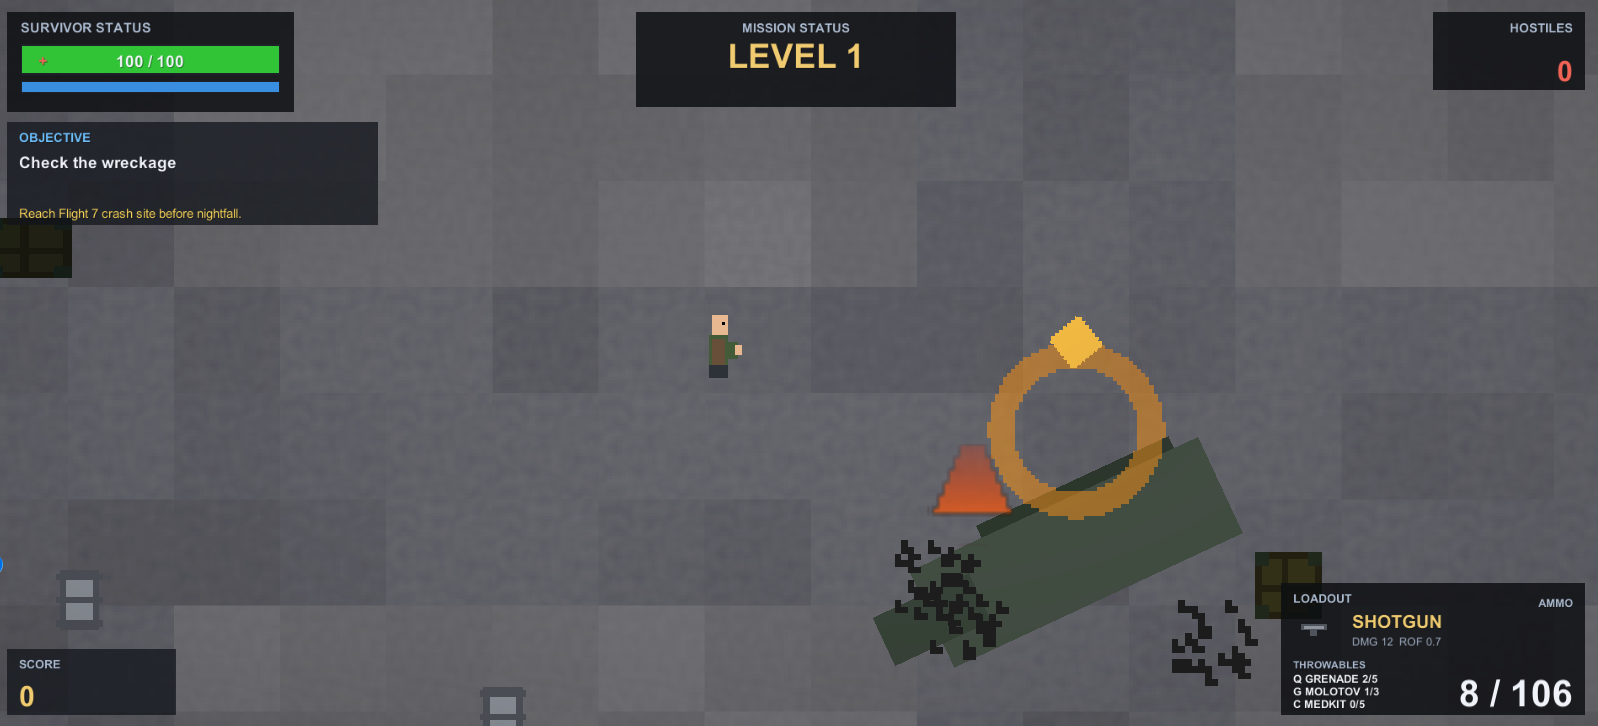
\includegraphics[width=\textwidth]{d2_fig_daytime.png}
    \caption{Supply crate loot prompt during the day phase. The interaction label appears only when the player is within range.}
  \end{subfigure}
  \hfill
  \begin{subfigure}[t]{0.48\textwidth}
    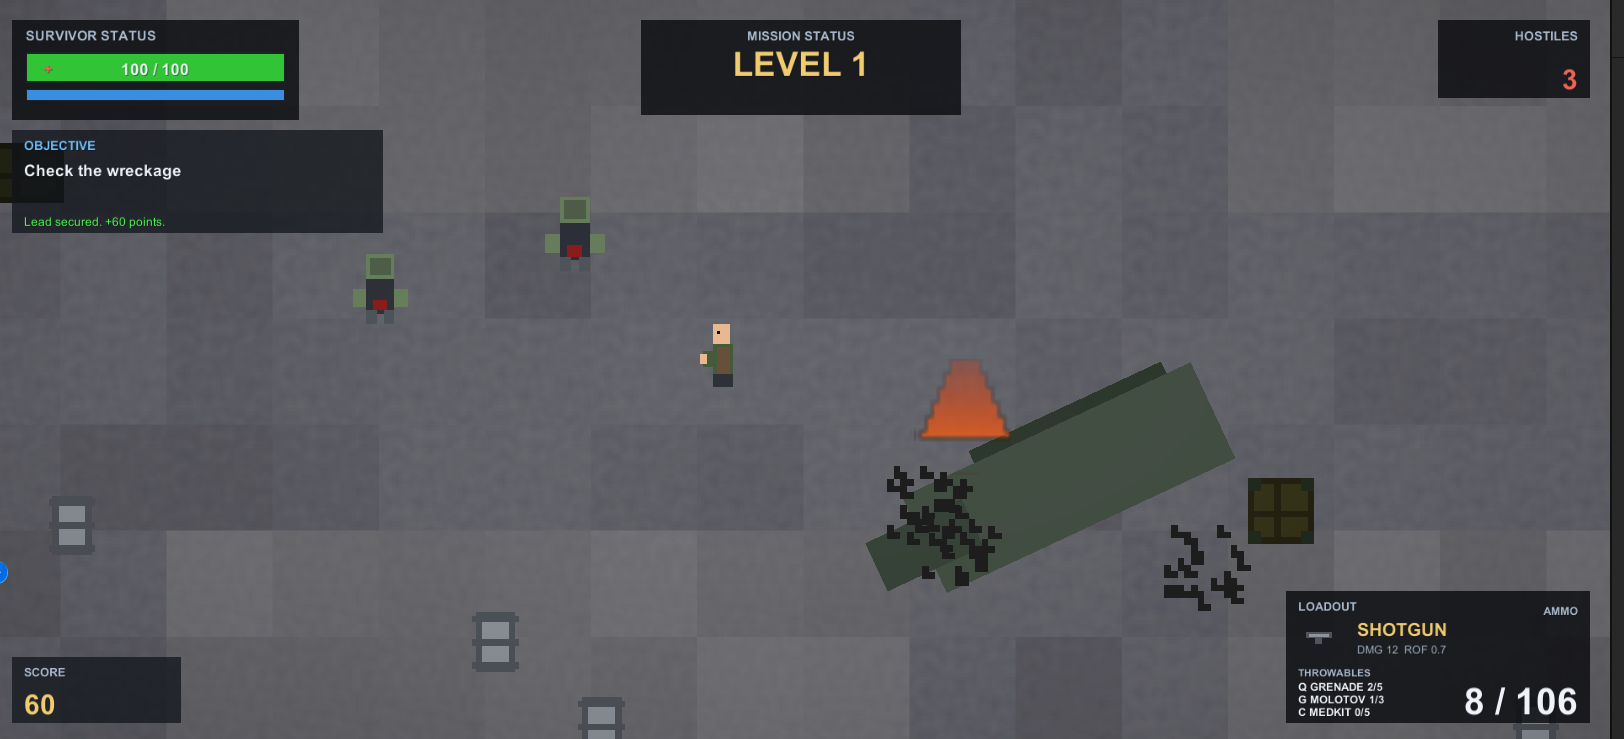
\includegraphics[width=\textwidth]{d2_fig_combat.png}
    \caption{Night combat with accumulated blood decals. Decals remain for the duration of the night.}
  \end{subfigure}
\end{figure}

% ===================================================================
%  6. TECHNICAL IMPLEMENTATION
% ===================================================================
\section{Technical Implementation}

\subsection{Architecture}

The project uses a set of singleton manager objects connected through C\# events. All managers are set to persist across scene loads using \texttt{DontDestroyOnLoad}. \texttt{GameManager} uses \texttt{[RuntimeInitializeOnLoadMethod]} to check for and create any missing managers at startup, so the build works correctly even if a manager object is missing from the scene.

\begin{center}
\small
\begin{tabular}{@{} l l @{}}
\toprule
\textbf{Manager} & \textbf{Responsibility} \\
\midrule
\texttt{GameManager} & State machine, level unlock and reset, player setup \\
\texttt{GameFlowController} & Day and night flow, pickup and crate spawning, drops \\
\texttt{DayNightCycle} & Per-night duration values, timer events \\
\texttt{WaveManager} & Wave schedules, enemy spawning, boss trigger \\
\texttt{NarrativeManager} & Dialogue queue, message protection, COMMS output \\
\texttt{StoryObjective} & Per-night story beats, day and night phase tracking \\
\texttt{AudioManager} & Music crossfade, tension mix, SFX pool, voice ducking \\
\texttt{ProgressionManager} & Milestone point awards and per-night stipends \\
\texttt{PointsSystem} & Score tracking and kill-streak multiplier \\
\texttt{RunModifierSystem} & Per-run and per-night modifier selection \\
\texttt{AtmosphereController} & Scene colour tint and weather effects \\
\texttt{VFXManager} & Screen shake, muzzle flash, particle effects \\
\bottomrule
\end{tabular}
\end{center}

\subsection{Game State Machine}

\texttt{GameManager.GameState} defines seven states that represent the full flow of a session.

\begin{center}
\texttt{MainMenu} $\to$ \texttt{DayPhase} $\to$ \texttt{NightPhase} $\to$ \texttt{DawnPhase} $\to$ \texttt{LevelComplete} $\to$ \texttt{Victory} \,/\, \texttt{GameOver}
\end{center}

Each state change fires the \texttt{OnGameStateChanged} C\# event. Systems such as \texttt{AudioManager}, \texttt{AtmosphereController}, and the UI panels subscribe to this event independently. New systems can respond to state changes without modifying \texttt{GameManager}.

\subsection{Procedural Map System}

Each level has a dedicated builder class (\texttt{TownCenterBuilder}, \texttt{SuburbanBuilder}, \texttt{IndustrialBuilder}, \texttt{ResearchBuilder}) that extends \texttt{MapBuilderBase}. These builders place buildings, roads, obstacles, spawn points, and lore props at runtime according to layout rules defined for each map. When the player moves to the next level, \texttt{TestSceneSetup.RebuildMap()} removes the old map and builds the new one within the same scene, so no scene load is needed and all manager state is preserved.

\subsection{Boss Fight}

\texttt{BossController} runs the Subject~23 encounter across three phases based on health thresholds.

\begin{itemize}[noitemsep]
  \item \textbf{Phase 1} (above 60\% health): The boss pursues the player using \texttt{SimpleEnemyAI}.
  \item \textbf{Phase 2} (30\% to 60\% health): The boss adds charge attacks at 12 units per second, dealing 40 damage on contact.
  \item \textbf{Phase 3} (below 30\% health): The boss adds a seismic slam attack with a 4-unit radius and 30 area damage.
\end{itemize}

When the boss is first activated, a coroutine runs a red screen flash and a 0.8-second screen shake, and the music switches to the boss track. The night does not end until \texttt{WaveManager.\-IsFinalBossDefeatedForCurrentNight()} returns true, which prevents the victory state from triggering before the boss is actually defeated.

\begin{figure}[H]
  \centering
  \begin{subfigure}[t]{0.48\textwidth}
    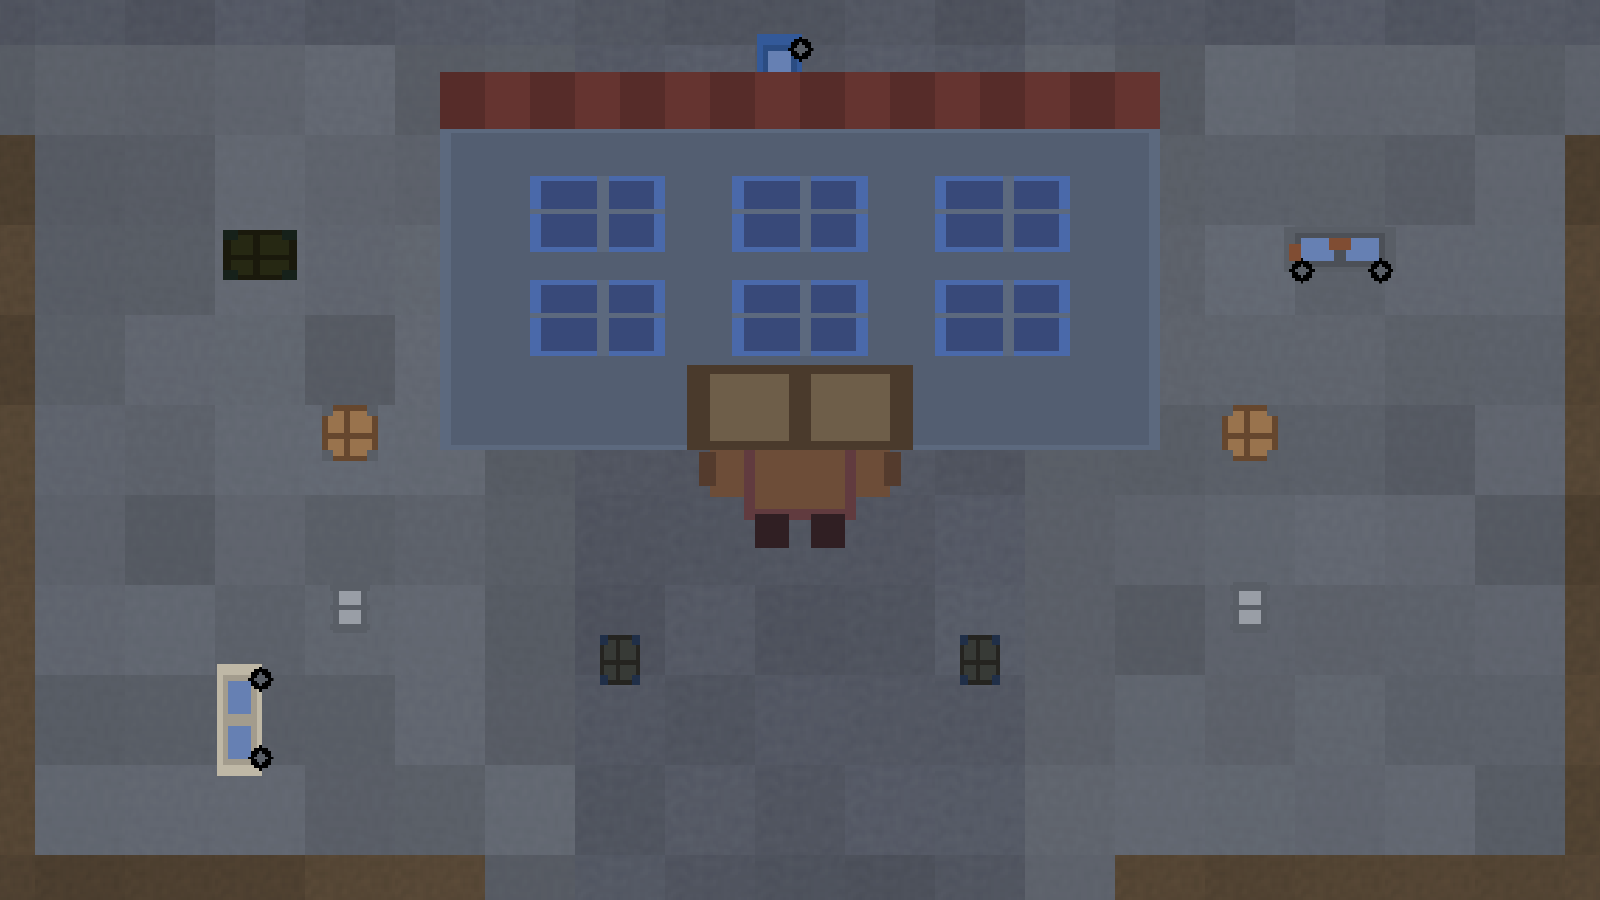
\includegraphics[width=\textwidth]{d3_fig_boss_fight.png}
    \caption{Boss-fight staging capture in the Level 4 main lab. Subject~23 marker and player position are shown in the final-night arena.}
  \end{subfigure}
  \hfill
  \begin{subfigure}[t]{0.48\textwidth}
    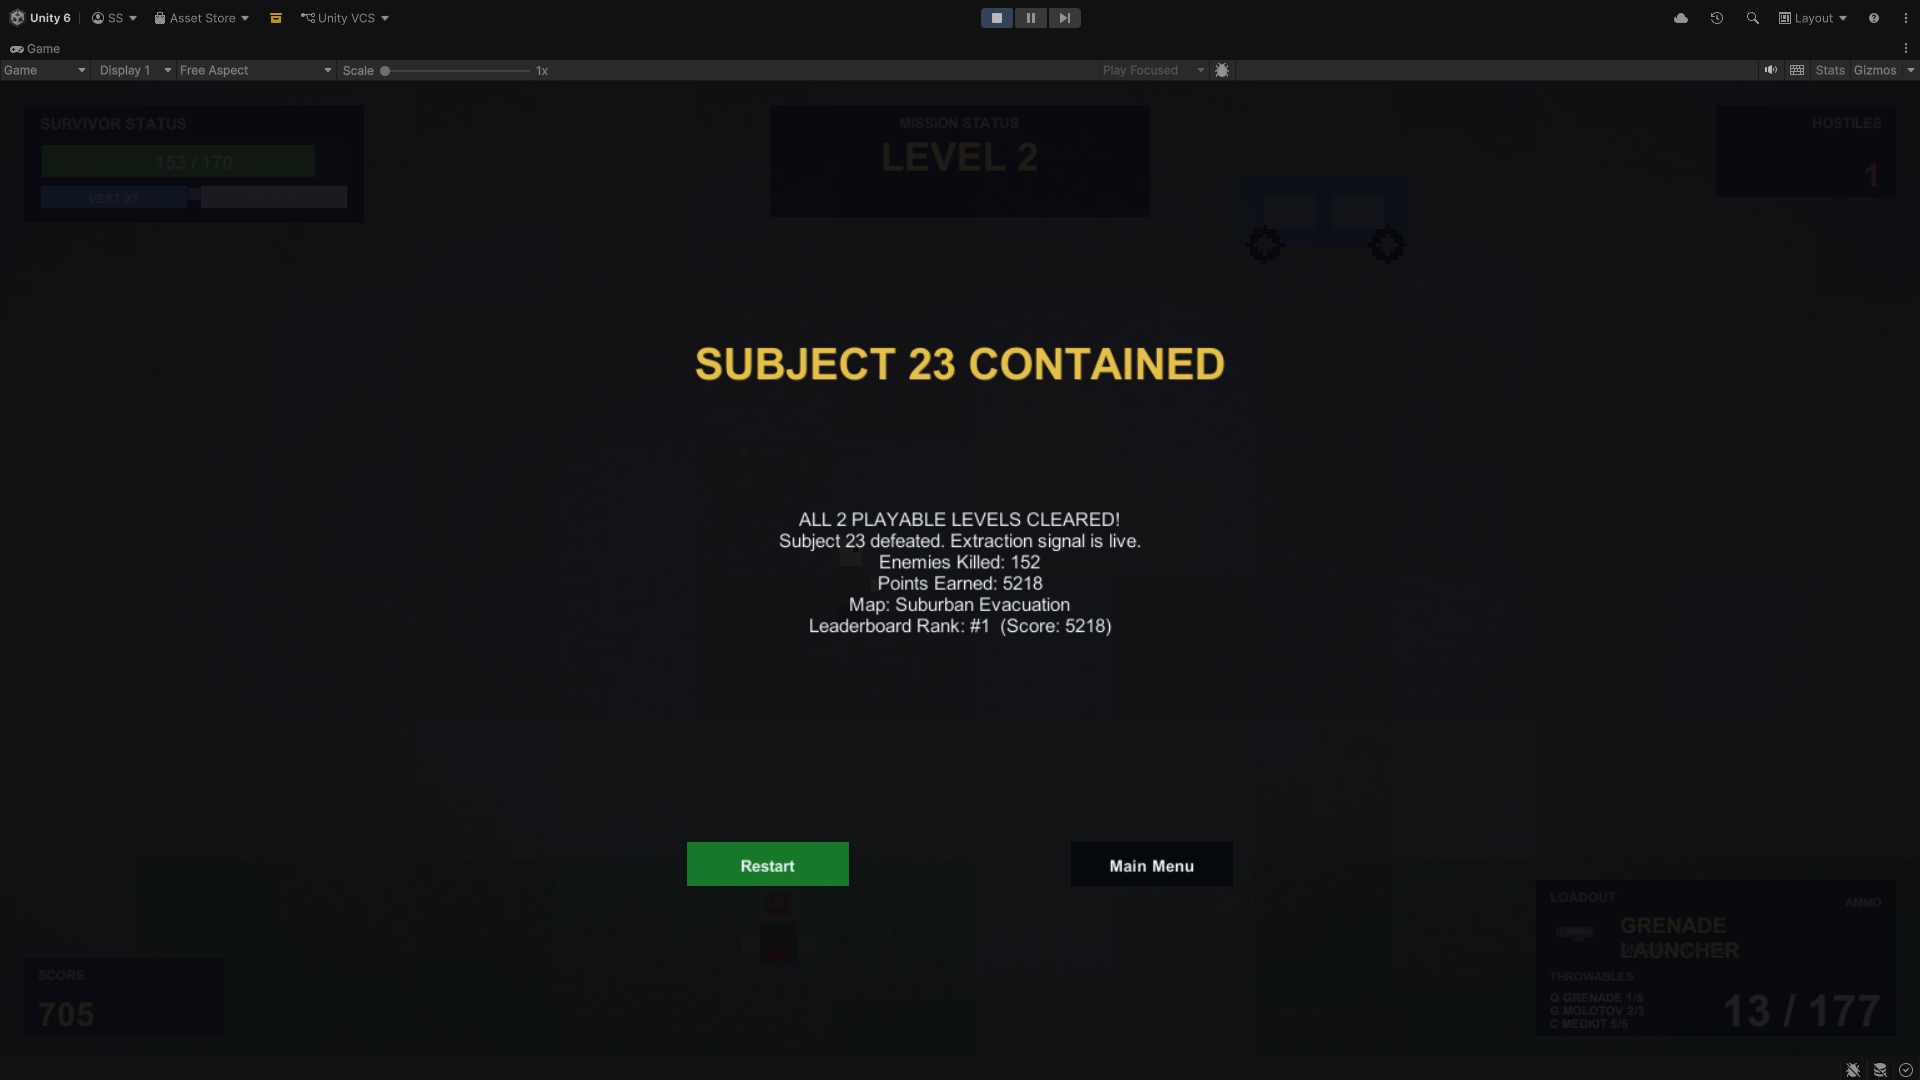
\includegraphics[width=\textwidth]{d2_fig_victory.png}
    \caption{Post-boss victory panel after Subject 23 defeat, including rank and run statistics.}
  \end{subfigure}
\end{figure}

\subsection{Code Patterns Used}

\begin{itemize}[noitemsep]
  \item \textbf{Observer pattern:} C\# events are used throughout (\texttt{OnGameStateChanged}, \texttt{OnNight\-Changed}, \texttt{OnContestedDropState\-Changed}, \texttt{OnDayTimerUpdate}, \texttt{OnDawnPhaseStarted}, and others).
  \item \textbf{Object pooling:} The audio system pre-allocates ten \texttt{AudioSource} components for spatial sound effects instead of creating and destroying them per sound.
  \item \textbf{Fallback handling:} All managers check for null before acting. The pickup placement function retries up to 100 times and falls back to a corner position if no valid spot is found, so placement never fails silently.
  \item \textbf{Singleton scope:} \texttt{DontDestroyOnLoad} is used only on manager objects. Enemy, bullet, and pickup objects are created and destroyed normally during gameplay.
\end{itemize}

% ===================================================================
%  7. CONCLUSION
% ===================================================================
\section{Conclusion}

\textit{Deadlight: Survival After Dark} is a complete four-level survival game that covers the core design principles from the course. The MDA framework is present throughout: the mechanics are the wave and economy loop; the dynamics are the risk and reward trade-offs during the day and night phases; and the intended player experience includes tension, exploration, and narrative engagement. The design accounts for different player priorities through adaptive resource scaling, optional lore collection, and a radio-based story arc.

The main additions in Deliverable 3 compared to Deliverable 2 are the completion of Levels 3 and 4, the boss encounter in the Research Facility, adaptive resource balancing informed by playtest observations, and the audio and visual polish pass. Each change was made in response to a specific problem identified during testing rather than added speculatively.

The game builds and runs as a Windows executable. All systems described in this report are active in the submitted build.

\end{document}
